
\section{Implementación de casos de estudio con servicios en la nube existente}
\label{\detokenize{chapter_two/study_cases_implementation:implementacion-de-casos-de-estudio-con-servicios-en-la-nube-existente}}\label{\detokenize{chapter_two/study_cases_implementation::doc}}


\subsubsection{Reconocimiento de rostros utilizando la API de Kairos}

En la arquitectura utilizamos los servicios de detección de rostros y reconocimiento
de sujetos de la API de Kairos.
Dentro de la aplicación móvil, la API REST de CloudNAO es el intermediario
que se comunica con la API de Kairos, esto es por facilidad y por no
tener que manejar muchas API y SDK por cada servicio que se desee usar.
A pesar de que en el sistema sólo se utiliza el servicio
dentro de la aplicación móvil, es posible ejecutar directamente la clase
\texttt{Kairos} del módulo \texttt{app.tpa\_client\_libraries.kairos\_client}
en el robot (esta clase es parte del la API REST de CloudNAO), para enviar la petición y procesar la respuesta desde éste.
Por ahora sólo se muestra el uso de este servicio en la aplicación móvil.

Cuando el usuario selecciona en el menú de navegación de la aplicación
la tarea de \textbf{Reconocimiento de personas} se muestra una pantalla 
con tres botones, uno para obtener una fotografía del robot, otro para
detectar rostros de nuevas personas, y el tercero para reconocer sujetos
ya almacenados. Si el usuario desea añadir a una nueva persona, se abre un
formulario emegente con un campo para agregar el nombre de la persona y
si no hay errores y la detección se realizó correctamente,
la cara de la persona queda almacenada y se pueden realizar futuros reconocimientos.

Si se desea realizar el reconocimiento de personas cuyo rostro
fue previamente guardado, se presiona el botón con la etiqueta
\textit{Reconoce personas} y si todo sale bien,
se muestra una lista de las personas en la fotografía.
Al dar clic sobre el nombre de la persona en la lista, el robot ejecuta
un movimiento de saludo diciendo una frase simple con el nombre de la persona.

\begin{figure}[!h]
\centering
\caption{El flujo de el reconocimiento de personas.}
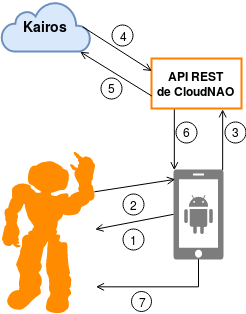
\includegraphics[scale=0.6]{study_case_kairos}
\end{figure}

\subsubsection{Reconocimiento óptico de caracteres con la API de Google Cloud Vision}

El reconocimiento óptico de caracteres (OCR por sus siglas en inglés) es 
el proceso de detectar y extraer texto de imágenes para luego
almacenarlo en un formato que una máquina pueda entender.
La API de Vision de Google Cloud ofrece el servicio de OCR
que además de incluye la detección del idioma en que se encuentra escrito


\paragraph{Traducción de texto encontrado en una imagen}

\subsubsection{Control por voz del robot con la API de Wit.ai}


Aquí debo describir cada elemento de la aplicación móvil
Descrito a detalle, cómo se combinan los servicios para que el robot
haga algo.

La detección  de rostros es un problema levemente resuelto por el equipo
de Aldebaran; existe un módulo dentro de NAOqi para seguir rostros o detectarlos,
así como reconocer algunos antes guardados. Sin embargo, los modelos de visión
que utilizan no son lo suficientemente potentes, ya que deben ejecutarse dentro
del robot. 

Recuerda ser más creativo para que no quede toda la tesis 
desproporcionada. Mover a los anexos si es necesario.
Agregar al capítulo 3 cosas de TF y DL.
